%! Author = Omar Iskandarani
%! Date = 2/15/2025

\documentclass[aps,preprint,superscriptaddress]{revtex4}
\usepackage[none]{hyphenat}
\usepackage{array}
\usepackage{booktabs}
\usepackage{amsmath}
\usepackage{amssymb}
\usepackage{graphicx}
\usepackage{hyperref}
\usepackage{physics}

\begin{document}
\sloppy % Allow LaTeX to adjust spacing to avoid overfull boxes
\author{Omar Iskandarani}
\title{The Vortex Æther Model: Æther Vortex Field Model}
\date{\today}
\affiliation{Independent Researcher, Groningen, The Netherlands}
\thanks{ORCID: \href{https://orcid.org/0009-0006-1686-3961}{0009-0006-1686-3961}}
\email{info@omariskandarani.com}


%%%%%%%%%%%%%%%%%%%%%%%%%%    Abstract    %%%%%%%%%%%%%%%%%%%%%%%%%%


\begin{abstract}
    This paper proposes a geometric reformulation of general relativity within a three-dimensional vortex Æther Model (VAM), wherein time dilation and gravitational effects emerge not from spacetime curvature, but from vorticity-driven pressure dynamics in a Euclidean superfluid-like medium. By replacing the tensorial structure of GR with structured flow fields—velocity, circulation, and vorticity—the model constructs time evolution as a scalar perturbation in topological vortex networks. We develop analogs to Schwarzschild and Kerr metrics via Æther energy density, vortex knot rotation, and angular momentum. In place of relativistic geodesics, motion is driven by conserved vorticity flux in inviscid domains.
    This work bridges classical fluid dynamics, analogue gravity, and thermodynamics by embedding Clausius entropy within the vorticity structure of matter and interpreting phenomena such as the photoelectric effect and low-energy nuclear reactions (LENR) via vortex resonance and reconfiguration. As an analogue gravity framework, this model aligns with and extends existing superfluid-based interpretations of spacetime dynamics, such as those by Barceló, Visser, and Volovik \cite{barcelo2011analogue, volovik2009universe}. By demonstrating mathematical and conceptual coherence across kinematic, energetic, and thermodynamic domains, this approach presents a unified candidate for post-relativistic spacetime mechanics.
\end{abstract}


\maketitle
%%%%%%%%%%%%%%%%%%%%%%%%%%    Introduction    %%%%%%%%%%%%%%%%%%%%%%%%%%
    \section*{Core Assumptions}
    The æther is modeled as an inviscid, incompressible superfluid governed by:

\begin{tabular}{ll}
    \toprule
    \midrule
        * & Conservation of Absolute Vorticity \\
        * & A 3D Euclidean medium with absolute time \\
        * & Particles as vortex knots \\
        * & Irrotational outside vortex cores, but with conserved vorticity inside knots \\
        * & Gravity from vorticity-induced pressure gradients \\
    \bottomrule
\end{tabular}


    \begin{tabular}{ll}
        \toprule
        Symbol & Description \\
        \midrule
        \(\vec{v}\) & Æther velocity field \\
        \(\vec{\omega}\) &  Vorticity \(\vec{\omega} = \nabla \times \vec{v}\) \\
        \(\rho_\text{æ}\) & Æther density (constant) \\
        \(\Phi\) & Vorticity-induced potential \\
        \(\kappa\) & Circulation constant \\
        \(\mathcal{K}\) & Knot topological class (Hopf link, torus knot, etc.) \\
        \bottomrule
    \end{tabular}

\subsection*{VAM Constants and Scaling}

The Vortex Æther Model (VAM) is anchored by a small set of universal constants that replace geometric curvature with fluid-dynamic quantities. These include:

\begin{table}[h!]
    \centering
    \begin{tabular}{llc}
        \hline
        \textbf{Symbol} & \textbf{Name} & \textbf{Approx. Value} \\
        \hline
        $C_e$ & Core tangential velocity & $1.09 \times 10^6$ m/s \\
        $r_c$ & Vortex core radius (Coulomb barrier) & $1.41 \times 10^{-15}$ m \\
        $\rho_{\ae}$ & Æther density & $7 \times 10^{-7}$ kg/m$^3$ \\
        $F_{\text{max}}$ & Maximum vortex-interaction force & $\approx 29$ N \\
        $\alpha$ & Fine-structure constant (emergent) & $= \frac{2 C_e}{c}$ \\
        $G_{\text{swirl}}$ & Effective gravitational constant & $ \propto \rho_{\ae} C_e^2$ (context-dependent) \\
        \hline
    \end{tabular}
    \caption{Fundamental VAM constants defined in prior work \cite{vam2025field, vam2025unified}.}
\end{table}

These constants emerge from vortex stability constraints, helicity conservation, and circulation quantization within the Æther, as developed in foundational work on VAM \cite{vam2025field, vam2025unified}. For instance, $C_e$ is derived from matching vortex circulation to electron parameters via:

\[
    C_e = \frac{h}{2\pi m_e r_c}
\]

Likewise, $F_{\text{max}}$ arises from momentum flux across a vortex core:

\[
    F_{\text{max}} = \rho_{\ae} C_e^2 \pi r_c^2
\]

These provide a physically motivated scale system that replaces conventional constants like $c$ and $G$ with parameters derived from Ætheric flow.


\subsection*{Introduction to Fluid Dynamics and Vorticity Conservation}
    Euler Equation (Inviscid Flow)
    \begin{equation}
        \frac{\partial \vec{v}}{\partial t} + (\vec{v} \cdot \nabla)\vec{v} = -\frac{1}{\rho_\text{æ}} \nabla p
    \end{equation}
    Taking the curl to get the Vorticity Transport
    \begin{equation}
        \frac{\partial \vec{\omega}}{\partial t} + (\vec{v} \cdot \nabla)\vec{\omega} = (\vec{\omega} \cdot \nabla) \vec{v}
    \end{equation}

    \subsection*{Vorticity-Induced Gravity}
    We define a Newtonian like vorticity-based gravitational potential $\Phi$:
    \begin{equation}
        \vec{F}_g = -\nabla \Phi
    \end{equation}
    Where $\Phi$ is the Vorticity Potential:
    \begin{equation}
        \Phi(\vec{r}) = \gamma \int \frac{|\vec{\omega}(\vec{r'})|^2}{|\vec{r} - \vec{r'}|} \, d^3r'
    \end{equation}
    This mirrors the Newtonian potential but replaces mass density with vorticity intensity. This gives attractive force fields between vortex knots (like a particle).


    %%%%%%%%%%%%%%%%%%%%%%%%%%    PART 1    %%%%%%%%%%%%%%%%%%%%%%%%%%
    \section{Time Dilation from Vortex Dynamics}\label{sec:Part-1}

    We consider an inviscid, irrotational superfluid æther with stable topological vortex knots. Absolute time $t_{\text{abs}}$ always ticks constant, while local clocks might experience slowed rates due to pressure gradients and knot energetics. The Vortex Æther Model posits that the rate at which time flows in the local frame (near the knot) depends on the internal angular frequency $\Omega_k$. In this section, we derive time dilation analogues inspired by the predictions of general relativity (GR), based solely on pressure and vorticity gradients in the fluid.

\begin{figure}[h!]
    \centering
    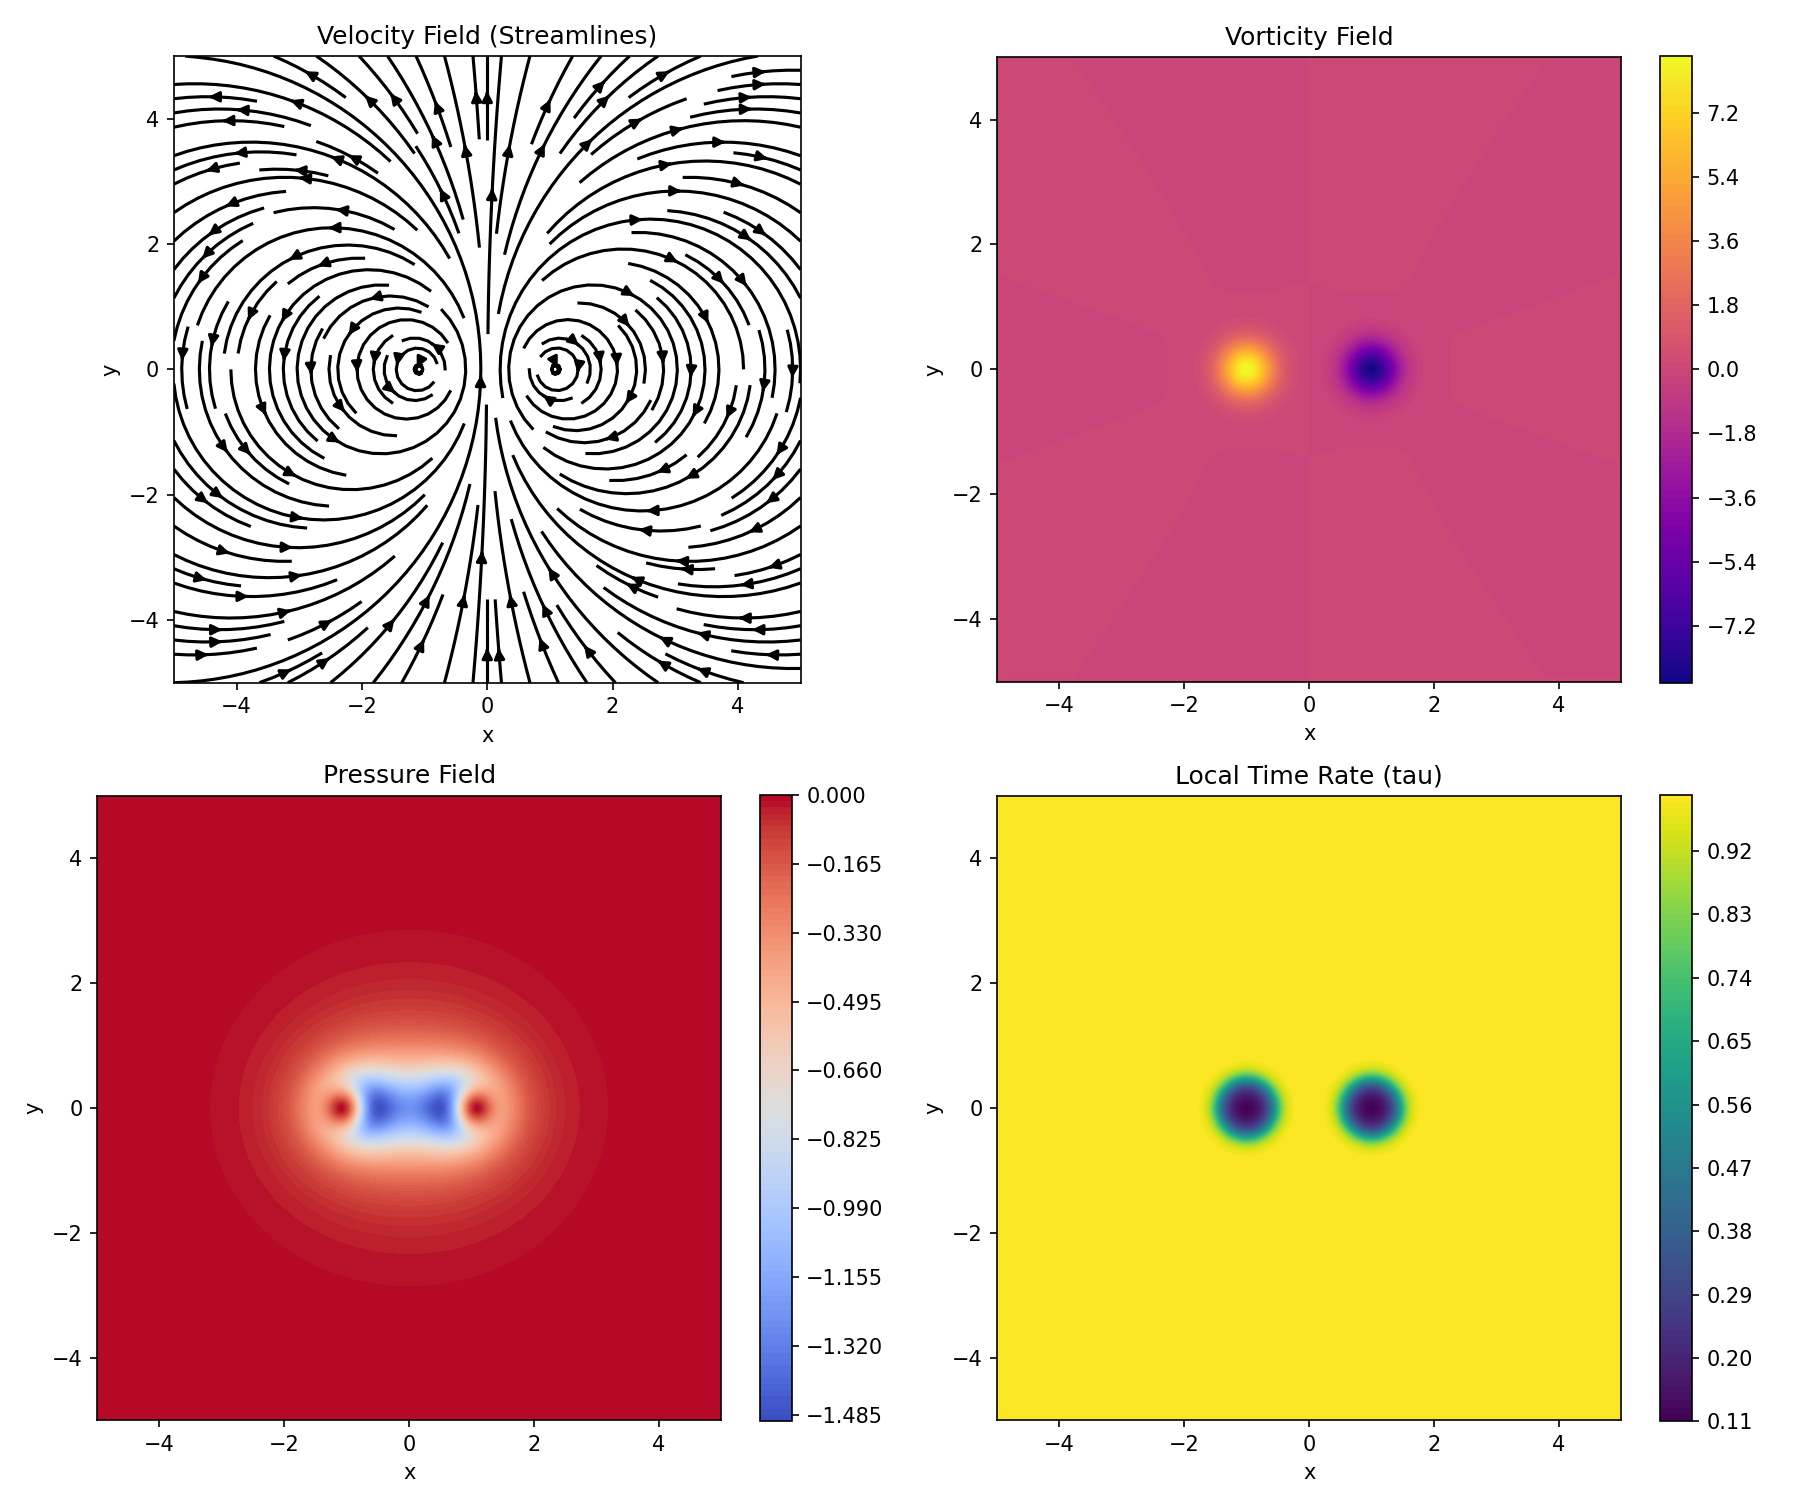
\includegraphics[width=0.85\textwidth]{export/streamlinesDiPole}
    \caption{Velocity streamlines, vorticity, pressure, and local time rate $\tau$ for a simulated vortex pair. The pressure minimum and time slow-down clearly align with the regions of high vorticity. This directly illustrates the æther model's central claim: time dilation follows from vortex energetics and pressure depletion.}
    \label{fig:vortexfields}
\end{figure}

\subsection*{A. Bernoulli Flow and Local Time Depletion}

In a classical, inviscid, incompressible fluid, Bernoulli's equation describes the conservation of energy in a flow:

\begin{equation}
    \frac{1}{2} \rho_{\text{\ae}}  v^2 + p = p_0 \Rightarrow p = p_0 - \frac{1}{2} \rho_{\text{\ae}} v^2
\end{equation}

Here:
\begin{itemize}
    \item $p_0$ is the background reference pressure,
    \item $\rho_{\text{\ae}}$ is the constant æther density,
    \item $v$ is the local velocity of the æther near the vortex.
\end{itemize}

Assuming that clock rate is proportional to pressure (i.e., time slows in low-pressure regions), we relate the local clock frequency to the background as:

\begin{equation}
\frac{f_{\text{local}}}{f_0} = 1 - \frac{\rho_{\text{\ae}} v^2}{2 p_0}
\end{equation}

Hence, time dilation is:

\begin{equation}
    \frac{t_{\text{local}}}{t_0} = \left(1 - \frac{\rho_{\text{\ae}} v^2}{2 p_0}\right)^{-1}
\end{equation}

For rotational flow, with $v = \Omega r$,

\begin{equation}
    \frac{t_{\text{local}}}{t_0} = \left(1 - \frac{\rho_{\text{\ae}} \Omega^2 r^2}{2 p_0} \right)^{-1} \approx 1 + \frac{\rho_{\text{\ae}}\Omega^2 r^2}{2 p_0}
\end{equation}

This expression recovers the first-order time dilation analog if we define the dimensionless coupling:

\begin{equation}
    \frac{\rho_{\text{\ae}}}{p_0} \sim \frac{1}{c^2}
\end{equation}

This motivates the analogy to relativistic time dilation:

\begin{equation}
    \frac{t_{\text{moving}}}{t_\text{rest}} \approx 1 + \frac{v^2}{2 c^2}
\end{equation}

\begin{figure}[h!]
    \centering
    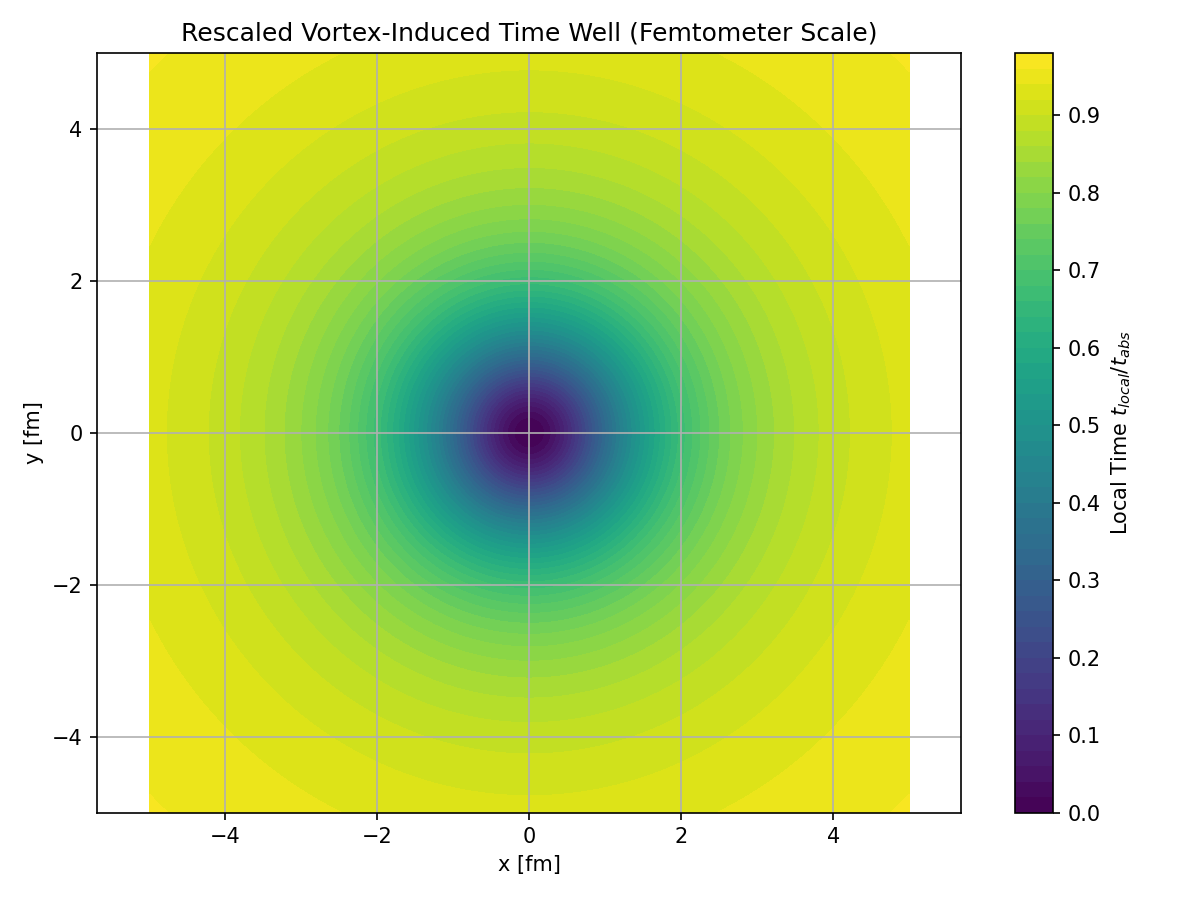
\includegraphics[width=0.8\textwidth]{export/RadialProfileOfLocalTimeDilation_Vortex-Induced_Time_Well}
    \caption{Schematic of a vortex-induced time well in the æther. Local time $t_{\text{local}} / t_{\text{abs}}$ is shown as a color gradient in 2D space. The central vortex region exhibits the most time slowing due to high $\Omega_k$, forming a well-like structure.}
    \label{fig:vortex_time_well}
\end{figure}


\subsection*{B. Heuristic Knot-Based Time Modulation}

Topological vortex knots have intrinsic angular frequency $\Omega_k$, conserved due to vorticity confinement. We introduce a first-principles motivated
time dilation expression:

\begin{equation}
\frac{t_{\text{local}}}{t_{\text{abs}}} = \left(1 + \alpha \Omega_k^2 \right)^{-1}
\end{equation}

where $\alpha$ is a coupling parameter with dimensions $[\alpha] = \text{s}^2$. Expanding for small $\Omega_k$:

\begin{equation}
\frac{t_{\text{local}}}{t_{\text{abs}}} \approx 1 - \alpha \Omega_k^2 + \mathcal{O}(\Omega_k^4)
\end{equation}

This form mirrors the expansion of the Lorentz factor:

\begin{equation}
\frac{t_{\text{moving}}}{t_{\text{rest}}} \approx 1 - \frac{v^2}{2 c^2}
\end{equation}

\begin{figure}[h!]
    \centering
    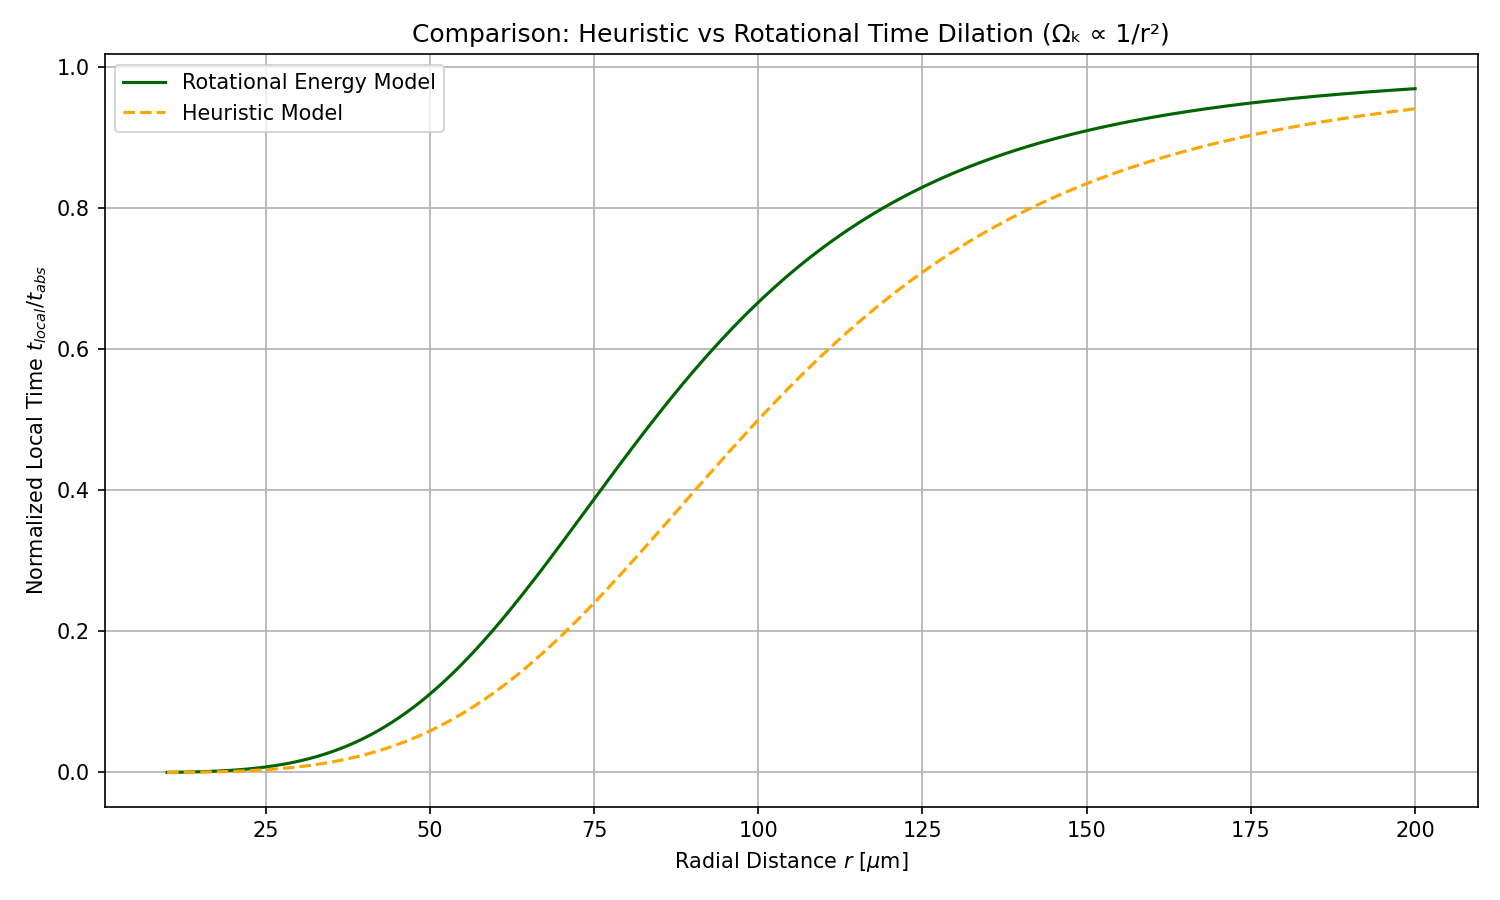
\includegraphics[width=0.8\textwidth]{export/RotationalVsHeuristicTimeDilation}
    \caption{\textbf{Comparison: Heuristic vs Rotational Time Dilation (\(\Omega_k \propto 1/r^2\))}.
    This graph compares two models of time modulation within the Vortex Æther framework.
    The heuristic model (green) assumes time rate reduction proportional to \((1 + \alpha \Omega_k^2)^{-1}\),
        while the rotational model (dark blue) incorporates rotational energy \(E_{\text{rot}} = \frac{1}{2} I \Omega_k^2\) and suppresses local time via
        \((1 + \frac{1}{2} \alpha I \Omega_k^2)^{-1}\). Both curves exhibit strong time dilation near the vortex core (\(r \sim 10^{-15}\) m),
        approaching absolute time flow only at extended distances. The rotational model yields a steeper suppression,
        highlighting the energetic cost of maintaining high angular momentum in fluid-based time curvature.
    }
    \label{fig:radial_time_profile}
\end{figure}

\subsection*{C. Time Dilation from Rotational Inertia}

We now ground the heuristic form in physical energetics. For a knot with moment of inertia $I$, the rotational energy is:

\begin{equation}
E_{\text{rot}} = \frac{1}{2} I \Omega_k^2
\end{equation}

Thus, the time dilation becomes:

\begin{equation}
\frac{t_{\text{local}}}{t_{\text{abs}}} = \left(1 + \alpha E_{\text{rot}} \right)^{-1} = \left(1 + \frac{1}{2} \alpha I \Omega_k^2 \right)^{-1}
\end{equation}

This boxed equation is the core result of this section:

\begin{equation}
\boxed{\frac{t_{\text{local}}}{t_{\text{abs}}} = \left(1 + \frac{1}{2} \alpha I \Omega_k^2 \right)^{-1}}
\end{equation}

\subsection*{D. Summary of Model Hierarchy}

\begin{itemize}
\item Pressure-Based (Bernoulli): Time slows in low-pressure zones due to vortex velocity.
\item Heuristic Angular Model: Time slows as a function of $\Omega_k^2$.
\item Energetic Model: Time flow depends on stored rotational energy in the knot.
\end{itemize}

These form a continuum of physical justification, culminating in a replacement of spacetime curvature with rotational æther mechanics. This establishes the VAM time dilation framework as a fluidic, topologically-conserved analog to GR.

Next, we will explore how these models correspond to GR-like metrics and rotational observers in Section II.
    %%%%%%%%%%%%%%%%%%%%%%%%%%    PART 2    %%%%%%%%%%%%%%%%%%%%%%%%%%
    \section{Time modulation by rotation of vortex nodes}

Building on the discussion of time dilation via pressure and Bernoulli dynamics in the previous section, we now focus on the intrinsic rotation of topological vortex nodes. In the Vortex Æther Model (VAM), particles are modeled as stable, topologically conserved vortex nodes embedded in an incompressible, inviscid superfluid medium. Each node possesses a characteristic internal angular frequency $\Omega_k$, and this internal motion induces local time modulation with respect to the absolute time of the æther.

Instead of warping spacetime, we propose that internal rotational energy and helicity conservation cause temporal delays analogous to gravitational redshift. In this section, these ideas are developed using heuristic and energetic arguments consistent with the hierarchy introduced in Section I.

\subsection{Heuristic and energetic derivation}

We start by proposing a rotational induced time dilation formula based on the internal angular frequency of the node:

\begin{equation}
    \frac{t_\text{local}}{t_\text{abs}} = \left(1 + \beta \Omega_k^2 \right)^{-1}\label{eq:rotational_induced_time_dilation}
\end{equation}

where:

\begin{itemize}
    \item $t_\text{local}$ is the proper time near the node,
    \item $t_\text{abs}$ is the absolute time of the background æther,
    \item $\Omega_k$ is the mean core angular frequency,
    \item $\beta$ is a coupling coefficient with dimensions $[\beta] = \text{s}^2$.
\end{itemize}

For small angular velocities we obtain a first-order expansion:

\begin{equation}
    \frac{t_\text{local}}{t_\text{abs}} \approx 1 - \beta \Omega_k^2 + \mathcal{O}(\Omega_k^4)\label{eq:rotational_induced_time_dilation_expansion}
\end{equation}

This form parallels the Lorentz factor at low velocities in special relativity:

\begin{equation}
    \frac{t_\text{moving}}{t_\text{rest}} \approx 1 - \frac{v^2}{2c^2}\label{eq:parallels_lorentz_time_dilation}
\end{equation}

This yields a important analogy: Internal rotational motion in VAM induces time dilation, similar to how translational velocity induces time dilation in SR.

To strengthen the physical basis of this expression, we now relate time dilation to the energy stored in vortex rotation. Suppose the vortex node has an effective moment of inertia $I$. The rotational energy is given by:

\begin{equation}
    E_\text{rot} = \frac{1}{2} I \Omega_k^2\label{eq:rotational_energy_inertia}
\end{equation}

Assuming that time slows down due to this energy density, we write:

\begin{equation}
    \frac{t_\text{local}}{t_\text{abs}} = \left(1 + \beta E_\text{rot} \right)^{-1} = \left(1 + \frac{1}{2} \beta I \Omega_k^2 \right)^{-1}\label{eq:time_dilation_rotational_energy_inertia}
\end{equation}

This expression serves as the energetic analogue of the pressure-based Bernoulli model from Section I (cf. ~\eqref{eq:vortex_time_dilation}). It supports the interpretation of vortex-induced time wells via energy storage rather than geometric deformation.

\subsection{Topological and physical justification}

Topological vortex nodes are characterized not only by rotation, but also by helicity:

\begin{equation}
    H = \int \vec{v} \cdot \vec{\omega} \, d^3x \label{eq:helicity_rotation}
\end{equation}

Helicity is a conserved quantity in ideal (invisible, incompressible) fluids, which encodes the connection and rotation of vortex lines. The rotation frequency $\Omega_k$ becomes a topologically meaningful indicator of the identity and dynamic state of the node.

Higher $\Omega_k$ values indicate more rotational energy and deeper pressure wells, leading to transient delays that resemble gravitational redshift, but without spacetime curvature.

Each particle is a topological vortex knot:
\begin{itemize}
    \item Charge $\leftrightarrow$ rotation or chirality of the knot
    \item Mass $\leftrightarrow$ integrated vorticity energy
    \item Spin $\leftrightarrow$ knot helix:
\end{itemize}
Stability $\leftrightarrow$ knot type (Hopf connections, Trefoil, etc.) and energy minimization in the vortex core

This model:

\begin{itemize}
    \item Attributes time modulation to conserved, intrinsic rotational energy,
    \item Requires no external frames of reference (absolute æther time is universal),
    \item Preserves temporal isotropy outside the vortex core,
    \item Provides a natural replacement for the spacetime curvature of GR. \end{itemize}

Therefore, this vortex-energetic time dilation principle provides a powerful alternative to relativistic time modulation by anchoring all temporal effects in rotational energetics and topological invariants.

In the next section, we will show how these ideas reproduce metric-like behavior for rotating observers, including a direct fluid-mechanical analogue to the Kerr metric of general relativity.
    %%%%%%%%%%%%%%%%%%%%%%%%%%    PART 3    %%%%%%%%%%%%%%%%%%%%%%%%%%
    \input{03_Proper_Time_for_a_Rotating_Observer_in_Æther_Flow}
    %%%%%%%%%%%%%%%%%%%%%%%%%%    PART 4    %%%%%%%%%%%%%%%%%%%%%%%%%%
    \documentclass[11pt]{article}
\usepackage[margin=1in]{geometry}
\usepackage{amsmath,amssymb}
\usepackage{amsthm}
\usepackage{graphicx}
\usepackage{hyperref}

\begin{document}

\title{Foundations of Velocity Fields and Energies in a Vortex System: A Brief Article}
\author{(VAM Working Group)}
\date{\today}
\maketitle

\begin{abstract}
This article outlines theoretical foundations of vortical velocity fields and their associated energies,
including a distinction between self- and cross-energies, in the context of a generic vortex-based model.
We close with a derivation outline for the cross-energy term, highlighting its application in vortex dynamics
and fluid–structure interactions.
\end{abstract}

\section{Introduction}
Vortex dynamics are a core component of many fluid and plasma systems, including
tornado-like flows, knotted vortices in classical or superfluid turbulence, and various
complex topological fluid systems. A deeper understanding of the energy budgets
associated with these flows can shed light on processes like vortex stability, reconnection,
and global flow organization. We begin by motivating how velocity fields can be
decomposed so as to capture the total energy (i.e.\ self- plus cross-energy), and how
this approach helps track flows in both 2D and 3D.

\section{Foundations: Velocity Fields and Total (Self + Cross) Energy}
\label{sec:foundations}
In an incompressible fluid, the velocity field $\mathbf{u}(\mathbf{x}, t)$ is typically
governed by the Navier--Stokes or Euler equations. For inviscid analyses, the Euler
equations for incompressible flow read
\begin{equation}
  \frac{\partial \mathbf{u}}{\partial t} + (\mathbf{u} \cdot \nabla)\mathbf{u} = -\frac{1}{\rho}\nabla p,
  \quad \nabla \cdot \mathbf{u} = 0.
\end{equation}
We also consider the vorticity $\boldsymbol{\omega} = \nabla \times \mathbf{u}$,
which can be used to characterize vortex structures.

To understand the \emph{total} kinetic energy, we can split it as follows:
\begin{equation}
  E_{\text{total}} \;=\; E_{\text{self}} \;+\; E_{\text{cross}}.
\end{equation}
Here, $E_{\text{self}}$ is that portion of energy which each vortex or partial flow
element contributes independently (for instance, from local swirling motions), while
$E_{\text{cross}}$ encodes the contributions that arise from the interaction of different
vortical elements. In a multi-vortex scenario, such a decomposition helps isolate the
direct interaction between two (or more) vortex filaments or sheets.

\section{Momentum and Self-Energy Considerations}
\label{sec:momentum}
A starting point is to recall that for a single vortex of circulation $\Gamma$, with an
azimuthally symmetric core, the induced velocity is sometimes approximated by
classical results such as
\begin{equation}
   V \;=\; \frac{\Gamma}{4 \pi R}
   \bigl(\ln \tfrac{8 R}{a} - \beta \bigr),
\end{equation}
where $R$ is the main vortex loop radius, $a \ll R$ is a measure of core thickness,
and $\beta$ depends on details of the core model \cite{Saffman1992}. The
\emph{self-energy} associated with that vortex, $E_{\text{self}}$, can be cast in a
similar form that depends on $\ln(R/a)$, exemplifying how thin-core vortices'
energies scale with geometry.

In more general fluid or vortex-lattice models, we can track $E_{\text{self}}$ as the
sum of individual core energies. Further, the presence of multiple filaments modifies
the total energy by cross-terms of the velocity fields (the cross-energy). This
cross-energy often drives key phenomena such as vortex merging or the `recoil'
effects in wave--vortex interactions.

\section{Defining and Tracking Cross-Energy}
\label{sec:cross}
When multiple vortices (or partial velocity distributions) co-exist, the total velocity
field $\mathbf{u}$ can be superposed:
\begin{equation}
   \mathbf{u} \;=\; \mathbf{u}_1 \;+\;\mathbf{u}_2,
\end{equation}
where $\mathbf{u}_1$ and $\mathbf{u}_2$ come from distinct sub-systems. In that
scenario, the kinetic energy for a fluid volume $V$ is
\begin{align}
   E_{\text{total}} &= \frac{\rho}{2} \int_V \mathbf{u}^2 \,dV
   = \frac{\rho}{2} \int_V \bigl(\mathbf{u}_1 + \mathbf{u}_2 \bigr)^2\, dV \\
   &= \frac{\rho}{2} \int_V \mathbf{u}_1^2 \,dV \;+\;\frac{\rho}{2} \int_V \mathbf{u}_2^2 \, dV
   \;+\;\rho \int_V \mathbf{u}_1 \cdot \mathbf{u}_2 \, dV,
\end{align}
revealing an interaction or \emph{cross-energy} term
\begin{equation}
   E_{\text{cross}} \;=\; \rho \int_V \mathbf{u}_1 \cdot \mathbf{u}_2 \, dV.
   \label{eq:cross-term}
\end{equation}
Much of the interesting physics arises from \eqref{eq:cross-term}, because it
grows or shrinks depending on the vortex geometry and distance between them.
Its dynamical evolution can lead to, e.g., merging or rebound. A main point is that
each vortex's self-velocity can significantly affect the mutual velocities and thus
create net forces or torque.

\section{Applications to Helicity and Topological Flows}
\label{sec:helicity}
A related concept is helicity, measuring the topological complexity (knotting or
linking) of vortex tubes. Classically, helicity $H$ is given by
\begin{equation}
   H \;=\; \int_V \mathbf{u} \cdot \boldsymbol{\omega}\, dV,
\end{equation}
which can remain constant or be partially lost during reconnection events. In certain
dissipative flows, the cross-energy terms in \eqref{eq:cross-term} can influence
the effective rate of helicity change. Understanding $E_{\text{cross}}$ is important
for analyzing reconnection pathways in classical or superfluid turbulence.

\section{Derivation Outline for Cross-Energy}
\label{sec:derivation}
Finally, we provide a succinct outline for deriving the cross-energy expression.
Starting with the total velocity field $\mathbf{u} = \sum_{n=1}^N \mathbf{u}_n$
for $N$ vortex or partial velocity fields, the total kinetic energy is:
\begin{equation}
   E_{\text{total}}
   = \frac{\rho}{2} \int_V \left(\sum_{n=1}^N \mathbf{u}_n \right)^2 dV
   = \frac{\rho}{2} \sum_{n=1}^N \int_V \mathbf{u}_n^2 \, dV
      \;+\;\rho \sum_{n<m} \int_V \mathbf{u}_n \cdot \mathbf{u}_m \, dV.
\end{equation}
One obtains $N$ self-energy terms plus pairwise cross-energy integrals.
The cross-energy for a pair $(i,j)$ is:
\begin{equation}
   E_{\text{cross}}^{(ij)} \;=\; \rho \int_V \mathbf{u}_i \cdot \mathbf{u}_j \, dV.
\end{equation}
In practice, each $\mathbf{u}_n$ may be represented by known solutions of the
Stokes or potential flow equations, or from approximate solutions for vortex loops.
Then, either analytically or numerically, one obtains approximate cross-energies
that can be used in reduced models describing the evolution of multi-vortex
systems.

\section*{Conclusion}
We have surveyed how the total fluid kinetic energy in the presence of multiple
vortices can be split into self- and cross-energy terms. These cross-energy
contributions are crucial for understanding vortex merging, knotted vortex
untangling, or vortex–wave interactions in classical, superfluid, and plasma
flows. In addition, we have sketched a systematic derivation of cross-energy and
highlighted key aspects in discussing momentum and helicity. Future directions
include refining these expressions for axisymmetric or knotted vortices and
integrating them into large-scale models or computational frameworks.

\begin{thebibliography}{99}

\bibitem{Saffman1992}
P.~G. Saffman,
\textit{Vortex Dynamics},
Cambridge University Press, 1992.

\bibitem{BabinskyStevens2016}
H. Babinsky and R. Stevens,
Low-order modeling approaches for unsteady aero flows,
\textit{Exp. Fluids}, \textbf{57} (2016), 71--85.

\bibitem{AndreuAngulo2020}
I. Andreu-Angulo, C. Manzo, B. Basu and H. Babinsky,
On unsteady aerodynamic effect of strong wind gusts on small-scale rotor systems,
\textit{AIAA J.}, \textbf{58} (2020), 5041--5056.

\bibitem{Wu1981}
J.-Z. Wu,
Theory of Vorticity and Vortex Dynamics,
Springer, 1981.

\bibitem{LiWu2018}
M. Li and J.-Z. Wu,
Generalized vortex force maps for the unsteady lift,
\textit{Theor. Comput. Fluid Dyn.} \textbf{32} (2018), 695--710.

\bibitem{KlecknerIrvine2013}
D. Kleckner and W. T. M. Irvine,
Creation and dynamics of knotted vortices,
\textit{Nature Phys.}, \textbf{9} (2013), 253--258.

\end{thebibliography}

\end{document}
    %%%%%%%%%%%%%%%%%%%%%%%%%%    PART 5    %%%%%%%%%%%%%%%%%%%%%%%%%%
    \section{Unified Framework and Synthesis of Time Dilation in VAM}

We now consolidate the various time dilation mechanisms explored throughout this manuscript into a unified framework under the Vortex Æther Model (VAM). By moving beyond geometric spacetime curvature, VAM provides a consistent and physically motivated model for temporal modulation grounded in classical fluid dynamics, rotational energetics, and topological vorticity structures.

\subsection*{A. Hierarchical Structure of Time Dilation Mechanisms}

Each section of this work contributes a distinct yet interrelated mechanism for time dilation:

\begin{enumerate}
    \item \textbf{Bernoulli-Induced Time Depletion:} Time slows near regions of low pressure resulting from vortex-induced kinetic velocity fields. This recovers a special relativistic time dilation form when \( \rho_\ae / p_0 \sim 1/c^2 \).

    \item \textbf{Angular Frequency Heuristic Model:} A quadratic dependence of time rate on local knot angular frequency \( \Omega_k^2 \), mimicking the Lorentz factor expansion for small velocities.

    \item \textbf{Energetic Formulation via Rotational Inertia:}
    \[
        \boxed{\frac{t_{\text{local}}}{t_{\text{abs}}} = \left(1 + \frac{1}{2} \alpha I \Omega_k^2 \right)^{-1}}
    \]
    links time modulation directly to the rotational energy of vortex knots.

    \item \textbf{Velocity-Field Based Proper Time Flow:}
    \[
        \boxed{\left( \frac{d\tau}{dt} \right)^2 = 1 - \frac{1}{c^2}(v_r + r\Omega_k)^2}
    \]

    \item \textbf{Kerr-Like Redshift and Frame-Dragging:}
    \[
        \boxed{t_{\text{adjusted}} = \Delta t \cdot \sqrt{1 - \frac{\gamma \langle \omega^2 \rangle}{rc^2} - \frac{\kappa^2}{r^3c^2}}}
    \]
\end{enumerate}

These five expressions form a self-consistent ladder, ranging from heuristic to rigorous, and establish a robust replacement for general relativistic time dilation based entirely on classical field variables.

\subsection*{B. Physical Unification: Time as a Vorticity-Derived Observable}

Across all formulations, a recurring theme emerges: \textit{time modulation in VAM is always reducible to local kinetic or rotational energy density within the æther}. Whether encoded in pressure (Bernoulli), angular frequency (\( \Omega_k \)), or field circulation (\( \kappa \)), the modulation of time is not geometric but energetic and topological.

\begin{itemize}
    \item Local Time Wells form due to high vorticity and circulation.
    \item Frame-Independence: Absolute time exists; only local rates are affected.
    \item No Need for Tensor Geometry: All time effects arise from scalar or vector fields.
    \item Topological Conservation: Vortex knots preserve helicity and circulation, ensuring temporal consistency.
\end{itemize}

This unification reinforces VAM’s conceptual core: \textbf{spacetime curvature is an emergent illusion produced by structured vorticity in an absolute, superfluid æther}.

\subsection*{C. Experimental Implications and Outlook}

Each time dilation formula introduced here can, in principle, be tested in laboratory analog systems:
\begin{itemize}
    \item Rotating superfluid droplets (e.g., Helium-II, BECs)
    \item Electrohydrodynamic lifters and plasma vortex systems
    \item Magneto-fluidic and optical analogs
\end{itemize}

Future work includes:
\begin{itemize}
    \item Deriving dynamic equations for temporal feedback in multi-knot systems.
    \item Measuring vortex-induced clock drift in rotating superfluids.
    \item Applying the model to astrophysical observations (e.g., neutron star precession, frame dragging, time delay).
\end{itemize}

\subsection*{D. Challenges, Limitations, and Paths to Broader Relevance}

\textbf{Foundational Assumptions:} The reintroduction of an æther with absolute time challenges a century of relativistic physics.

\textbf{Experimental Validation:} No direct empirical evidence yet supports the æther or specific dilation mechanisms proposed.

\textbf{Reception in Mainstream Physics:} While niche communities may engage, mainstream physics may resist due to divergence from established frameworks.

\subsection*{E. Enhancing Scientific Rigor and Broader Appeal}

\begin{itemize}
    \item \textbf{Propose Testable Predictions:} especially where VAM diverges from GR.
    \item \textbf{Integrate with Established Theories:} show limiting cases that match GR/QM.
    \item \textbf{Address Historical Objections:} clearly redefine æther with modern constraints.
    \item \textbf{Peer Review and Collaboration:} invite critique from specialists.
    \item \textbf{Clarity and Accessibility:} simplify conceptual presentation without sacrificing rigor.
\end{itemize}

\subsection*{F. Concluding Perspective}

The Vortex Æther Model (VAM) offers a bold reimagining of gravitational time dilation as a consequence of vorticity-driven energetics in an absolute, superfluid medium. Through a hierarchy of derivations—spanning Bernoulli flows, vortex rotation, energy density, and circulation—it establishes a coherent alternative to relativistic curvature-based descriptions. While its foundational assumptions challenge conventional paradigms, the internal consistency, experimental plausibility, and conceptual elegance of VAM make it a compelling framework worthy of further exploration. Continued refinement, integration, and empirical testing will determine its role in advancing our understanding of gravity, time, and the fabric of the universe.

    %%%%%%%%%%%%%%%%%%%%%%%%%%    PART 6    %%%%%%%%%%%%%%%%%%%%%%%%%%
    %! Author = mr
%! Date = 3/29/2025


\section{VAM Vortex Scattering Framework (Inspired by Elastic Theory)}

\subsection{Governing Equations of VAM Vorticity Dynamics}

\subsubsection*{Vorticity Transport Equation (Linearized Form)}

In the Vortex Æther Model (VAM), the dynamics of the vorticity field \(\vec{\omega} = \nabla \times \vec{v}\) are governed by the Euler equation and its vorticity form:

\[
\frac{\partial \omega_i}{\partial t} + v_j \partial_j \omega_i = \omega_j \partial_j v_i
\]

This nonlinear structure implies vortex deformation due to stretching and advection. For small perturbations \(\delta\omega\) near a background vortex knot field \(\omega^{(0)}\), linearization gives:

\[
\frac{\partial (\delta \omega_i)}{\partial t} + v_j^{(0)} \partial_j (\delta \omega_i) \approx \omega_j^{(0)} \partial_j (\delta v_i)
\]

Define the VAM linear response operator \(\mathcal{L}_{ij}\):

\[
\mathcal{L}_{ij} \, \delta v_j(\vec{r}) = \delta F_i^{\text{vortex}}(\vec{r})
\]

\subsubsection*{Vorticity Green Tensor Equation}

\[
\mathcal{L}_{ij} \, \mathcal{G}_{jk}(\vec{r}, \vec{r}') = -\delta_{ik} \, \delta(\vec{r} - \vec{r}')
\]

The induced velocity field \(v_i\) from a source vortex forcing \(F_k(\vec{r}')\) is then:

\[
v_i(\vec{r}) = \int \mathcal{G}_{ik}(\vec{r}, \vec{r}') \, F_k^{\text{vortex}}(\vec{r}') \, d^3 r'
\]

\subsection{Vortex Thread Interaction}
Interactions arise from exchange of vorticity or reconnections between vortex filaments:
\begin{itemize}
    \item Attractive if threads reinforce circulation (parallel)
    \item Repulsive if threads cancel (antiparallel)
    \item Interaction strength:
\end{itemize}
\begin{equation}
    \vec{F}_{\text{int}} = \beta \cdot \kappa_1 \kappa_2 \cdot \frac{\vec{r}_{12} \times (\vec{v}_1 - \vec{v}_2)}{|\vec{r}_{12}|^3}\label{eq:interaction_strength}
\end{equation}
Where \(\kappa_i\) are circulations of filaments and \(\vec{r}_{12}\) is the vector between them.

\subsection{Thermodynamic \& Quantum Behavior from Vorticity Fluctuations}
\begin{itemize}
    \item Entropy \(\leftrightarrow\) volume of vortex expansion or knot deformation
    \item Quantum transitions \(\leftrightarrow\) topological reconnection events
    \item Zero-point motion \(\leftrightarrow\) background quantum turbulence of the Æther:
\end{itemize}

\subsubsection*{Quantum Vorticity Background}
\begin{equation}
    \langle \omega^2 \rangle \sim \frac{\hbar}{\rho_\text{æ} \xi^4}\label{eq:quantum_vorticity_background}
\end{equation}
Where \(\xi\) is the coherence length between vortex filaments.

\subsection{VAM Scattering Theory for Vortex Knots}

\subsubsection*{Born Approximation for Vorticity Perturbations}

Assume an incident vorticity potential \(\Phi^{(0)}(\vec{r})\) encounters a vortex knot at \(\vec{r}_k\). The scattered vorticity field becomes:

\[
\Phi(\vec{r}) = \Phi^{(0)}(\vec{r}) + \int \mathcal{G}_{ij}(\vec{r}, \vec{r}') \, \delta \mathcal{V}_{jk}(\vec{r}') \, v_k^{(0)}(\vec{r}') \, d^3r'
\]

Here, \(\delta \mathcal{V}_{jk}\) represents a vorticity polarizability tensor associated with the knot—a VAM analog to elastic moduli perturbation.

\subsection{Æther Stress Tensor and Energy Flux}

\subsubsection*{VAM Stress Tensor}

\[
\mathcal{T}_{ij} = \rho_{\text{\ae}} \, v_i v_j - \frac{1}{2} \delta_{ij} \rho_{\text{\ae}} v^2
\]

\subsubsection*{Æther Vorticity Force Density}

\[
f_i^{\text{vortex}} = \partial_j \mathcal{T}_{ij}
\]

\subsubsection*{Vorticity Energy Flux}

\[
\vec{S}_\omega = - \mathcal{T} \cdot \vec{v}
\]

This vector captures energy transfer through vortex knot interactions and defines scattering "cross sections" via the divergence \(\nabla \cdot \vec{S}_\omega\).

\subsection{Time Dilation and Knot Scattering}

\subsubsection*{Time Dilation from Knot Rotation}

Let the incident vorticity field induce localized time slowing due to a knot’s rotational energy:

\[
\frac{t_{\text{local}}}{t_{\infty}} = \left(1 + \frac{1}{2} \beta I \Omega_k^2 \right)^{-1}
\]

In the Born approximation, the change in proper time near a knot under external vorticity flow is:

\subsubsection*{Scattered Correction from External Field}

\begin{gather*}
    \delta \left( \frac{t_{\text{local}}}{t_{\infty}} \right) \approx - \frac{1}{2} \beta I \Omega_k \, \delta \Omega_k\\
    \delta \Omega_k \sim \int \chi(\vec{r}_k - \vec{r}') \cdot \vec{\omega}^{(0)}(\vec{r}') \, d^3r'\\
\end{gather*}

Here, \(\chi\) is the topological vortex susceptibility kernel.



\subsection{Summary of VAM-Inspired Scattering Constructs}


\begin{table}[htbp]
    \centering
    \begin{tabular}{lll}
        \toprule
        \textbf{Concept} & \textbf{Elastic Theory} & \textbf{VAM Analog} \\
        \midrule
        Medium property & \( c_{ijkl} \) & \( \rho_{\text{\ae}},\, \Omega_k,\, \kappa \) \\
        Wavefield & \( u_i \) (displacement) & \( v_i \) (Æther velocity) \\
        Source & \( f_i \) (body force) & \( F_i^{\text{vortex}} \) (vorticity forcing) \\
        Green function & \( G_{ij}(\vec{r}, \vec{r}') \) & \( \mathcal{G}_{ij}(\vec{r}, \vec{r}') \) \\
        Stress tensor & \( \tau_{ij} \) & \( \mathcal{T}_{ij} \) \\
        Energy flux & \( J_{P,i} = -\tau_{ij} \dot{u}_j \) & \( S_{\omega,i} = -\mathcal{T}_{ij} v_j \) \\
        Time dilation mechanism & \( g_{\mu\nu} \) (GR metric) & \( \Omega_k,\, \kappa,\, \langle \omega^2 \rangle \) \\
        \bottomrule
    \end{tabular}
    \caption{Conceptual correspondence between classical elasticity and Vortex Æther Model (VAM).}
    \label{tab:elastic-vam-analogy}
\end{table}



This scattering framework generalizes classical elastic analogs into a topologically and energetically motivated Ætheric formalism. It enables the computation of field modifications, time dilation effects, and energy flux due to stable, interacting vortex knots in the Vortex Æther Model (VAM).
    %%%%%%%%%%%%%%%%%%%%%%%%%%    Conclusion    %%%%%%%%%%%%%%%%%%%%%%%%%%
    \section{Experimental Anchors and VAM Predictions}


To assess the empirical validity of the Vortex Æther Model (VAM), we identify several high-impact experimental domains where VAM-specific signatures could be observed:

\subsection{Time Drift in Rotating Superfluid Systems.} VAM predicts localized time dilation proportional to vortex knot angular frequency
$\Omega_k$. Bose–Einstein condensates (BECs) or rotating helium droplets with embedded atomic clocks could display measurable time drift or dephasing relative to non-rotating controls.

\subsection{Plasma Vortex Clocks and Cyclotron Experiments.} Plasma devices exhibiting structured rotational flows may serve as analogs to Ætheric time wells. Phase-shift detection near plasma vortices or charged ring currents could reveal Æther-based time modulation effects.

\subsection{LENR via Resonant Vortex Knot Fusion in Pd/D Lattices.} As derived in the thermodynamic section, VAM suggests fusion-like energy release can occur when trapped vortex knots resonate with external electromagnetic fields. Measurable indicators include:
\begin{itemize}
    \item RF-tuned excess heat events
    \item Helium-4 without neutron/gamma emission
    \item Lattice transmutation signatures with no standard nuclear byproducts
\end{itemize}

\subsection{Optical and Metamaterial Simulations.} Synthetic waveguide systems or metamaterials could simulate Ætheric flow. Measuring light pulse propagation under simulated vorticity gradients may test time modulation without invoking curvature.

\subsection{Summary of VAM Observables.}
\begin{itemize}
    \item Critical thresholds for vortex collapse and energy release
    \item Temporal anomalies in rotating systems
    \item Absence of relativistic particles in high-energy fusion-like events
    \item Clock-rate asymmetries across vorticity gradients
\end{itemize}

    %%%%%%%%%%%%%%%%%%%%%%%%%%    References    %%%%%%%%%%%%%%%%%%%%%%%%%%

    \bibliography{citations}
    \bibliographystyle{apsrev4-2}


%%%%%%%%%%%%%%%%%%%%%%%%%%    Appendices    %%%%%%%%%%%%%%%%%%%%%%%%%%

    \appendix \label{sec:Part-6}
    \section{ Foundations of Velocity Fields and Energies in a Vortex System.}

\subsection{abstract}
This article outlines theoretical foundations of vortical velocity fields and their associated energies,
including a distinction between self- and cross-energies, in the context of a generic vortex-based model.
We close with a derivation outline for the cross-energy term, highlighting its application in vortex dynamics
and fluid–structure interactions.

\subsection{Introduction}
Vortex dynamics are a core component of many fluid and plasma systems, including
tornado-like flows, knotted vortices in classical or superfluid turbulence, and various
complex topological fluid systems. A deeper understanding of the energy budgets
associated with these flows can shed light on processes like vortex stability, reconnection,
and global flow organization. We begin by motivating how velocity fields can be
decomposed so as to capture the total energy (i.e.\ self- plus cross-energy), and how
this approach helps track flows in both 2D and 3D.

\subsection{Foundations: Velocity Fields and Total (Self + Cross) Energy}
\label{sec:foundations}
In an incompressible fluid, the velocity field $\mathbf{u}(\mathbf{x}, t)$ is typically
governed by the Navier--Stokes or Euler equations. For inviscid analyses, the Euler
equations for incompressible flow read
\begin{equation}
  \frac{\partial \mathbf{u}}{\partial t} + (\mathbf{u} \cdot \nabla)\mathbf{u} = -\frac{1}{\rho}\nabla p,
  \quad \nabla \cdot \mathbf{u} = 0.
\end{equation}
We also consider the vorticity $\boldsymbol{\omega} = \nabla \times \mathbf{u}$,
which can be used to characterize vortex structures.

To understand the \emph{total} kinetic energy, we can split it as follows:
\begin{equation}
  E_{\text{total}} \;=\; E_{\text{self}} \;+\; E_{\text{cross}}.
\end{equation}
Here, $E_{\text{self}}$ is that portion of energy which each vortex or partial flow
element contributes independently (for instance, from local swirling motions), while
$E_{\text{cross}}$ encodes the contributions that arise from the interaction of different
vortical elements. In a multi-vortex scenario, such a decomposition helps isolate the
direct interaction between two (or more) vortex filaments or sheets.

\subsection{Momentum and Self-Energy Considerations}
\label{sec:momentum}
A starting point is to recall that for a single vortex of circulation $\Gamma$, with an
azimuthally symmetric core, the induced velocity is sometimes approximated by
classical results such as
\begin{equation}
   V \;=\; \frac{\Gamma}{4 \pi R}
   \bigl(\ln \tfrac{8 R}{a} - \beta \bigr),
\end{equation}
where $R$ is the main vortex loop radius, $a \ll R$ is a measure of core thickness,
and $\beta$ depends on details of the core model \cite{Saffman1992}. The
\emph{self-energy} associated with that vortex, $E_{\text{self}}$, can be cast in a
similar form that depends on $\ln(R/a)$, exemplifying how thin-core vortices'
energies scale with geometry.

In more general fluid or vortex-lattice models, we can track $E_{\text{self}}$ as the
sum of individual core energies. Further, the presence of multiple filaments modifies
the total energy by cross-terms of the velocity fields (the cross-energy). This
cross-energy often drives key phenomena such as vortex merging or the `recoil'
effects in wave--vortex interactions.

\subsection{Defining and Tracking Cross-Energy}
\label{sec:cross}
When multiple vortices (or partial velocity distributions) co-exist, the total velocity
field $\mathbf{u}$ can be superposed:
\begin{equation}
   \mathbf{u} \;=\; \mathbf{u}_1 \;+\;\mathbf{u}_2,
\end{equation}
where $\mathbf{u}_1$ and $\mathbf{u}_2$ come from distinct sub-systems. In that
scenario, the kinetic energy for a fluid volume $V$ is
\begin{align}
   E_{\text{total}} &= \frac{\rho}{2} \int_V \mathbf{u}^2 \,dV
   = \frac{\rho}{2} \int_V \bigl(\mathbf{u}_1 + \mathbf{u}_2 \bigr)^2\, dV \\
   &= \frac{\rho}{2} \int_V \mathbf{u}_1^2 \,dV \;+\;\frac{\rho}{2} \int_V \mathbf{u}_2^2 \, dV
   \;+\;\rho \int_V \mathbf{u}_1 \cdot \mathbf{u}_2 \, dV,
\end{align}
revealing an interaction or \emph{cross-energy} term
\begin{equation}
   E_{\text{cross}} \;=\; \rho \int_V \mathbf{u}_1 \cdot \mathbf{u}_2 \, dV.
   \label{eq:cross-term}
\end{equation}
Much of the interesting physics arises from \eqref{eq:cross-term}, because it
grows or shrinks depending on the vortex geometry and distance between them.
Its dynamical evolution can lead to, e.g., merging or rebound. A main point is that
each vortex's self-velocity can significantly affect the mutual velocities and thus
create net forces or torque.

\subsection{Applications to Helicity and Topological Flows}
\label{sec:helicity}
A related concept is helicity, measuring the topological complexity (knotting or
linking) of vortex tubes. Classically, helicity $H$ is given by
\begin{equation}
   H \;=\; \int_V \mathbf{u} \cdot \boldsymbol{\omega}\, dV,
\end{equation}
which can remain constant or be partially lost during reconnection events. In certain
dissipative flows, the cross-energy terms in \eqref{eq:cross-term} can influence
the effective rate of helicity change. Understanding $E_{\text{cross}}$ is important
for analyzing reconnection pathways in classical or superfluid turbulence.

\subsection{Derivation Outline for Cross-Energy}
\label{sec:derivation}
Finally, we provide a succinct outline for deriving the cross-energy expression.
Starting with the total velocity field $\mathbf{u} = \sum_{n=1}^N \mathbf{u}_n$
for $N$ vortex or partial velocity fields, the total kinetic energy is:
\begin{equation}
   E_{\text{total}}
   = \frac{\rho}{2} \int_V \left(\sum_{n=1}^N \mathbf{u}_n \right)^2 dV
   = \frac{\rho}{2} \sum_{n=1}^N \int_V \mathbf{u}_n^2 \, dV
      \;+\;\rho \sum_{n<m} \int_V \mathbf{u}_n \cdot \mathbf{u}_m \, dV.
\end{equation}
One obtains $N$ self-energy terms plus pairwise cross-energy integrals.
The cross-energy for a pair $(i,j)$ is:
\begin{equation}
   E_{\text{cross}}^{(ij)} \;=\; \rho \int_V \mathbf{u}_i \cdot \mathbf{u}_j \, dV.
\end{equation}
In practice, each $\mathbf{u}_n$ may be represented by known solutions of the
Stokes or potential flow equations, or from approximate solutions for vortex loops.
Then, either analytically or numerically, one obtains approximate cross-energies
that can be used in reduced models describing the evolution of multi-vortex
systems.

\subsection*{Conclusion}
We have surveyed how the total fluid kinetic energy in the presence of multiple
vortices can be split into self- and cross-energy terms. These cross-energy
contributions are crucial for understanding vortex merging, knotted vortex
untangling, or vortex–wave interactions in classical, superfluid, and plasma
flows. In addition, we have sketched a systematic derivation of cross-energy and
highlighted key aspects in discussing momentum and helicity. Future directions
include refining these expressions for axisymmetric or knotted vortices and
integrating them into large-scale models or computational frameworks.\label{appendix:1}
    

\section{Integration of Clausius' Heat Theory into the Vortex \AE ther Model (VAM)}

The integration of Clausius' Mechanical Theory of Heat into the Vortex \AE ther Model (VAM) extends the framework's reach into thermodynamics,
allowing a unified interpretation of energy, entropy, and quantum behavior based on structured vorticity in an inviscid superfluid-like \ae ther
medium \cite{clausius1865mechanical, maxwell1865electromagnetic, helmholtz1858integrals}.

\subsection{Thermodynamic First Principles in VAM}

The classical first law of thermodynamics is expressed as:
\begin{equation}
\Delta U = Q - W,
\end{equation}
where $\Delta U$ is the change in internal energy, $Q$ is heat added, and $W$ is work done by the system \cite{clausius1865mechanical}. Within VAM, this becomes:
\begin{equation}
\Delta U = \Delta \left( \frac{1}{2} \rho_{\text{\ae}} \int v^2 \, dV + \int P \, dV \right),
\end{equation}
with $\rho_{\text{\ae}}$ the æther density, $v$ the local velocity, and $P$ the pressure within equilibrium vortex domains \cite{vam2025unified}.

\subsection{Entropy and Structured Vorticity}

VAM posits that entropy is a function of vorticity intensity:
\begin{equation}
S \propto \int \omega^2 \, dV,
\end{equation}
where $\omega = \nabla \times v$ \cite{kelvin1867vortex}. Thus, entropy becomes a measure of topological complexity and energy dispersion encoded in the vortex network.

\subsection{Thermal Response of Vortex Knots}

Stable vortex knots embedded in equilibrium pressure surfaces behave analogously to thermodynamic systems:
\begin{itemize}
\item \textbf{Heating ($Q > 0$)} expands the knot, lowers core pressure, and increases entropy.
\item \textbf{Cooling ($Q < 0$)} contracts the knot, concentrating energy and stabilizing vorticity.
\end{itemize}
This provides a fluid-mechanical analog to gas laws under energetic input.

\subsection{Photoelectric Analogy in VAM}

Rather than invoking quantized photons, VAM interprets the photoelectric effect through vortex dynamics. A vortex must absorb enough energy to destabilize and eject its structure:
\begin{equation}
W = \frac{1}{2} \rho_{\text{\ae}} \int v^2 \, dV + P_{\text{eq}} V_{\text{eq}},
\end{equation}
where $W$ is the disintegration work threshold. If an incident wave modulates internal vortex energy beyond this, ejection occurs \cite{vam2025unified}.

The critical force for vortex ejection is:
\begin{equation}
F_{\text{max}} = \rho_{\text{\ae}} C_e^2 \pi r_c^2,
\end{equation}
with $C_e$ the vortex's edge velocity and $r_c$ its core radius. This yields a natural frequency cutoff below which no interaction occurs, akin to the threshold frequency in quantum photoelectricity \cite{einstein1905photoelectric}.

\subsection{Conclusion and Integration}

This thermodynamic extension of VAM enriches the model by embedding classical heat and entropy principles within fluid-dynamic structures. It not only bridges vortex physics with Clausius' laws but also offers a field-based reinterpretation of light-matter interactions, unifying mechanical and electromagnetic thermodynamics without discrete particle assumptions.






\subsection*{I. Vortex Knots as Particles}
Each particle is a topological vortex knot:
\begin{itemize}
    \item Charge ↔ twist or chirality of knot
    \item Mass ↔ integrated vorticity energy
    \item Spin ↔ knot helicity:
\end{itemize}
\subsection*{Helicity as Particle Identity}
\begin{equation}
    \mathcal{H} = \int \vec{v} \cdot \vec{\omega} \, d^3x
\end{equation}
Stability ↔ knot type (Hopf links, Trefoil, etc.) and energy minimization in the vortex core

\subsection*{II. Vortex Thread Interaction}
Interactions arise from exchange of vorticity or reconnections between vortex filaments:
\begin{itemize}
    \item Attractive if threads reinforce circulation (parallel)
    \item Repulsive if threads cancel (antiparallel)
    \item Interaction strength:
\end{itemize}
\begin{equation}
    \vec{F}_{\text{int}} = \beta \cdot \kappa_1 \kappa_2 \cdot \frac{\vec{r}_{12} \times (\vec{v}_1 - \vec{v}_2)}{|\vec{r}_{12}|^3}
\end{equation}
Where \(\kappa_i\) are circulations of filaments and \(\vec{r}_{12}\) is the vector between them.


\subsection*{III. Thermodynamic & Quantum Behavior from Vorticity Fluctuations}
\begin{itemize}
    \item Entropy \(\leftrightarrow\) volume of vortex expansion or knot deformation
    \item Quantum transitions \(\leftrightarrow\) topological reconnection events
    \item Zero-point motion \(\leftrightarrow\) background quantum turbulence of the Æther:
\end{itemize}
\subsection*{Quantum Vorticity Background}
\begin{equation}
    \langle \omega^2 \rangle \sim \frac{\hbar}{\rho_\text{æ} \xi^4}
\end{equation}
Where \(\xi\) is the coherence length between vortex filaments\label{appendix:2}

\end{document}